% ============================================================
% main.tex — Quantum Encoding Benchmark on IQM Garnet QPU
% Author  : Rania Derouich
% ORCID   : https://orcid.org/0009-0009-6157-2647
% Compile : pdflatex main.tex  (×2)
%
% Fixes applied in v2 (CORRECTED):
%   1. Single \email split into two \email{} calls (arXiv format)
%   2. Abstract em-dashes restored (--- not removed by compiler)
%   3. Eq. (3) QAOA split onto two lines for two-column readability
%   4. GitHub URL fixed as single \url{} — no line-break in the middle
%   5. ORCID as clickable \href in Data Availability
%   6. \affiliation{Independent Researcher, Tunisia} added
%   7. Bowles 2024 benchmark citation added to Related Work
%   8. QPU total wall time sentence added to Results
%   9. IQP label note removed from body text (artefact to fix in figure)
%  10. Table I ref Angle RX fixed: schuld2022 → schuld2021kernel (PRL 2019)
%  11. \usepackage{xurl} added for clean URL line-breaking
%  12. ORCID \href: \texttt{} removed to fix clickable link in revtex4-2
%
% Additional fixes applied in v3 (FINAL — submission-ready):
%  13. RMSE unified to 3.314 throughout (abstract, conclusion) — was 3.31
%  14. IQP truncation note removed from Results body text (belongs in figure only)
%  15. QAOA-inspired circuit diagram added (TikZ) as Fig. 3 — reviewer request
%  16. Acknowledgments updated: 280 IQM Resonance credits from
%      "Simulating Complex Materials with Quantum Chemistry and SQD" workshop
%  17. \usepackage{tikz} + decorations.pathreplacing added for circuit figure
%  18. \qrisp{} macro used in Acknowledgments (was plain "Qrisp")
%
% Additional fixes applied in v4 (ARXIV-READY):
%  19. \bibitem{schuld2022} (orphaned) now cited in §Discussion NISQ context
%  20. Supplementary Material pointer added to Data Availability section
% ============================================================
\documentclass[twocolumn,aps,pra,superscriptaddress,floatfix]{revtex4-2}

% ── Packages ─────────────────────────────────────────────────
\usepackage[utf8]{inputenc}
\usepackage[T1]{fontenc}
\usepackage{amsmath,amssymb,amsfonts}
\usepackage{graphicx}
\usepackage{xcolor}
\usepackage{hyperref}
\usepackage{xurl}        % FIX 11 — clean URL breaks after / without breaking links
\usepackage{booktabs}
\usepackage{multirow}
\usepackage{array}
\usepackage{microtype}
\usepackage{siunitx}
\usepackage{physics}
\usepackage{tikz}
\usetikzlibrary{decorations.pathreplacing,calligraphy}

\hypersetup{
  colorlinks = true,
  linkcolor  = blue!70!black,
  citecolor  = blue!70!black,
  urlcolor   = blue!70!black
}

% ── Custom commands ───────────────────────────────────────────
\newcommand{\qrisp}{\textsc{Qrisp}}
\newcommand{\iqm}{\textsc{IQM}}
\newcommand{\gdsc}{\textsc{GDSC2}}
\newcommand{\ic}{\ensuremath{\text{IC}_{50}}}
\newcommand{\cobyla}{\textsc{COBYLA}}
\newcommand{\expvz}{\ensuremath{\langle Z_0 \rangle}}

% ─────────────────────────────────────────────────────────────
\begin{document}

% ── Title & author ────────────────────────────────────────────
\title{Quantum Encoding Strategies for Drug Response Prediction:\\
       An Exhaustive Benchmark on a 20-Qubit Superconducting QPU}

\author{Rania Derouich}
\email{derouichrania38@gmail.com}
\email{raniaderouich@ensi-uma.tn}
\affiliation{Independent Researcher, Tunisia}

\date{\today}

% ── Abstract ─────────────────────────────────────────────────
\begin{abstract}
We present the first systematic, hardware-executed benchmark of twelve distinct
quantum data-encoding strategies for drug-response prediction on a real
superconducting quantum processing unit~(QPU).
All experiments were conducted on the \iqm{} Garnet 20-qubit QPU via the
\iqm{} Resonance cloud platform, using the \qrisp{} quantum-software
framework~(v\,0.8.2).
Each encoding was evaluated on $n=50$ stratified samples drawn from the
Genomics of Drug Sensitivity in Cancer dataset (GDSC2, 242\,036
drug--cell-line pairs), targeting the natural-log IC$_{50}$ response variable.
Variational weights were optimised offline with the gradient-free \cobyla{}
algorithm before hardware submission.
Every circuit was executed with 1024~shots; the regression signal is the
zero-qubit Pauli expectation value $\expvz$.
Results show that the \textbf{QAOA-inspired} encoding achieves the best
RMSE of~$3.314$ and is statistically superior ($p<0.05$, Wilcoxon signed-rank
test) to six of the remaining eleven encodings.
% FIX 2 — em-dashes around parenthetical
Hardware-efficient entanglement structures---specifically alternating cost and
mixer layers---provide a systematic advantage over purely rotational or diagonal
encodings under realistic noise conditions.
This work constitutes a reproducible baseline for noise-aware quantum machine
learning on pharmaceutical data; all code, data, and raw QPU outputs are
publicly released.
\end{abstract}

\maketitle

% ─────────────────────────────────────────────────────────────
\section{Introduction}
\label{sec:intro}
% ─────────────────────────────────────────────────────────────

The capacity of quantum computers to manipulate exponentially large Hilbert
spaces has motivated extensive theoretical work on quantum machine learning
(QML)~\cite{biamonte2017,schuld2021,cerezo2021}.
A central open question is \emph{which data-encoding strategy} best exploits the
available quantum resources for a given supervised-learning task.
The encoding, or feature map, is the quantum circuit $\mathcal{U}(x)$ that
embeds a classical input $x\in\mathbb{R}^d$ into the quantum state space;
it fundamentally shapes the effective kernel of the variational
model~\cite{schuld2021kernel,havlicek2019}.

Previous benchmarks comparing encoding strategies have relied either on
classical simulators~\cite{perezSalinas2020,lloyd2020,killoran2019} or
on demonstrations limited to two to four
qubits~\cite{havlicek2019,mitarai2018}.
Simulators cannot reproduce the decoherence, gate error, and readout-noise
profiles of physical hardware, making hardware results essential for validating
the practical utility of any encoding.

Drug-response prediction estimating the sensitivity of a cancer cell line to
a given compound is a high-value bioinformatics task with direct clinical
relevance~\cite{iorio2016}.
The GDSC dataset provides a large-scale, publicly available regression benchmark
with continuous targets (LN-IC$_{50}$) over a biologically diverse feature
space, making it well suited for evaluating quantum regression pipelines.

\textbf{Contributions.}  This paper makes the following contributions:
\begin{enumerate}
  \item The first hardware benchmark of twelve quantum encoding strategies on a
        20-qubit superconducting QPU for a real pharmaceutical regression task.
  \item A complete, reproducible experimental pipeline from dataset
        preprocessing to QPU execution to statistical analysis built on the
        open-source \qrisp{} framework.
  \item Statistical comparison via the Wilcoxon signed-rank test,
        demonstrating that QAOA-inspired encoding achieves significant
        improvement over six of eleven competitors.
  \item Public release of all code, raw QPU measurements, and trained weights.
\end{enumerate}

% ─────────────────────────────────────────────────────────────
\section{Background}
\label{sec:background}
% ─────────────────────────────────────────────────────────────

\subsection{Variational Quantum Circuits for Regression}

A variational quantum circuit~(VQC) is composed of a data-dependent encoding
layer $\mathcal{U}(x)$ followed by a trainable ansatz $V(\theta)$:
\begin{equation}
  \ket{\psi(x,\theta)} = V(\theta)\,\mathcal{U}(x)\ket{0}^{\otimes n}.
\end{equation}
The prediction is obtained by measuring the expectation value of an observable
$\hat{O}$,
\begin{equation}
  f(x,\theta) = \bra{\psi(x,\theta)}\hat{O}\ket{\psi(x,\theta)},
\end{equation}
and mapping $f$ to the target domain via an affine transformation.
In this work, $\hat{O} = Z_0$ (Pauli-$Z$ on qubit~0) and the affine map
recovers the LN-IC$_{50}$ scale from $\expvz\in[-1,1]$.

\subsection{The Role of the Encoding}

Schuld and Killoran~\cite{schuld2021kernel} showed that a VQC effectively
implements a kernel function $\kappa(x,x')$ determined by the encoding.
Highly expressive encodings with multi-body interactions (e.g.\ ZZ-feature-map,
IQP) generate richer kernels but require deeper circuits that are more
susceptible to noise~\cite{wang2021noise}.
The optimal encoding is therefore hardware- and task-dependent.

% ─────────────────────────────────────────────────────────────
\section{Hardware and Software Platform}
\label{sec:platform}
% ─────────────────────────────────────────────────────────────

\subsection{IQM Garnet QPU}

All experiments were executed on the \iqm{} Garnet processor, a 20-qubit
superconducting QPU exposed through the \iqm{} Resonance cloud platform.
The native two-qubit gate is the controlled-$Z$~(CZ) gate; single-qubit
gates ($R_x$, $R_y$, $R_z$) are decomposed automatically.
The qubit topology is a crystal lattice with nearest-neighbour connectivity.
Each circuit was submitted with 1024~shots; the average per-sample execution
latency was $3.47\pm0.09$\,s, including queuing and classical post-processing.

\subsection{Qrisp Framework}

\qrisp{}~\cite{qrisp2024} is an open-source, high-level quantum programming
framework that provides a Python-native gate API and transparent backend
routing.
Circuits were constructed as \texttt{QuantumVariable} objects; execution used
\texttt{qv.get\_measurement(backend=quantum\_computer, shots=1024)}, which
returns a probability dictionary.
The expectation value $\expvz$ was computed analytically from the returned
shot counts.

% ─────────────────────────────────────────────────────────────
\section{Dataset and Preprocessing}
\label{sec:data}
% ─────────────────────────────────────────────────────────────

\subsection{GDSC2}

The Genomics of Drug Sensitivity in Cancer dataset (release~8.5, October~2023)
contains fitted dose-response curves for 286~drugs across 969~cancer cell
lines, totalling 242\,036 drug--cell-line pairs~\cite{iorio2016}.
The regression target is the natural-log half-maximal inhibitory concentration
$\text{LN\_IC}_{50}\in[-8.75,\,13.82]$.

Eight features were selected: area-under-the-curve~(AUC), RMSE of the
dose-response fit, Z-score, drug identifier, COSMIC cell-line identifier, and
three cancer-type binary flags (UNCLASSIFIED, LUAD, SCLC).
These features span pharmacological, genomic, and phenotypic dimensions while
remaining within the $d=8$ qubit budget.

Figure~\ref{fig:dataset} illustrates the LN-IC$_{50}$ distribution over the
full GDSC2 dataset, the QPU-sampled range, and the standardised feature matrix
for the 50 selected samples.

\begin{figure}[ht]
  \centering
  
\includegraphics[width=\columnwidth]{GDSC2_dataset_overview.png}
  \caption{%
    \textbf{GDSC2 dataset overview.}
    \textit{Left:} LN-IC$_{50}$ distribution over all 242\,036 pairs.
    Orange dashed lines delimit the QPU subset range $[-5.80,\,6.35]$;
    orange dots mark the 50 selected samples.
    \textit{Right:} Standardised feature matrix ($z$-score) for the
    50 QPU samples.  Features F1--F5 are continuous pharmacological
    descriptors; F6--F8 are binary cancer-type flags.
  }
  \label{fig:dataset}
\end{figure}

\subsection{Stratified QPU Sampling}

Quantum cloud execution is credit-constrained; we therefore drew $n=50$
samples using percentile-stratified sampling over $\text{LN\_IC}_{50}$
(10~bins, 5~samples/bin), ensuring full coverage of the response range
$[-5.80,\,6.35]$ in the QPU subset (Fig.~\ref{fig:dataset}, left).

\subsection{QuantumPreprocessor}

Input features were scaled to $[-\pi,\pi]$ for angle, phase, and Fourier
encodings via min-max normalisation.
Amplitude encoding additionally applies $\ell_2$ normalisation to map the
feature vector to the unit sphere.
Basis encoding discretises features to integer indices.
The LN-IC$_{50}$ target was mapped to $[-1,1]$ for $\expvz$-based regression,
with the inverse affine map applied at inference time.

% ─────────────────────────────────────────────────────────────
\section{Encoding Strategies}
\label{sec:encodings}
% ─────────────────────────────────────────────────────────────

We define twelve encoding functions $\mathcal{U}_k(x)$, $k=1,\ldots,12$,
each followed by an identical variational ansatz of $L=2$ layers.
Every layer consists of $R_y(\theta_{l,i,0})R_z(\theta_{l,i,1})$ on each
qubit, followed by a nearest-neighbour CZ ladder.
Table~\ref{tab:encodings} summarises the circuits; detailed circuit
definitions are available in the companion repository.

\begin{table}[ht]
\centering
\caption{%
  Summary of the twelve evaluated quantum encodings.
  $n_Q$ denotes the qubit count.
  ``This work'' indicates encodings introduced in this study.
}
\label{tab:encodings}
\renewcommand{\arraystretch}{1.15}
\begin{tabular}{@{}clcc@{}}
\toprule
\textbf{\#} & \textbf{Encoding} & $n_Q$ & \textbf{Ref.} \\
\midrule
1  & Angle RX              & 8 & \cite{schuld2021kernel} \\ % FIX 10 — was schuld2022 (wrong paper)
2  & Angle RY+RZ           & 8 & \cite{perezSalinas2020} \\
3  & Amplitude             & 4 & \cite{mottonen2004} \\
4  & Basis                 & 3 & \cite{nielsen2010} \\
5  & ZZ Feature Map        & 8 & \cite{havlicek2019} \\
6  & IQP                   & 8 & \cite{shepherd2009} \\
7  & Hamiltonian (Trotter) & 8 & \cite{lloyd2020} \\
8  & QAOA-inspired         & 8 & \cite{farhi2014} \\
9  & Squeezing (DV)        & 8 & \cite{killoran2019} \\
10 & Hybrid (Ang.+Amp.)    & 8 & This work \\
11 & Displacement (CV-DV)  & 8 & This work \\
12 & Data Re-uploading     & 8 & \cite{perezSalinas2020} \\
\bottomrule
\end{tabular}
\end{table}

\paragraph{QAOA-inspired encoding (best performer).}
Each of the $L$ layers alternates a \emph{cost} layer---phase gates
$R_z(2\gamma_i)$ driven by the data features $\gamma_i = x_i$---with a
\emph{mixer} layer of uniform $R_x(2\beta)$ rotations whose angle $\beta$
is a trainable parameter.
% FIX 3 — Equation split on two lines for two-column readability
\begin{align}
  \mathcal{U}_\text{QAOA}(x)
    &= \prod_{l=1}^{L}
       \underbrace{\bigotimes_{i}R_x(2\beta_l)}_{\text{mixer}}
       \nonumber\\
    &\quad\cdot
       \underbrace{\mathrm{CZ}_\text{ladder}
                   \cdot\bigotimes_{i}R_z(2x_i)}_{\text{cost}},
\end{align}
initialised from $\ket{+}^{\otimes n}$.
The alternating structure distributes the data-encoding more uniformly across
the circuit depth, reducing the concentration of errors on any single layer.
Figure~\ref{fig:qaoa_circuit} illustrates the single-layer structure for three
representative qubits.

\begin{figure*}[!t]
\centering
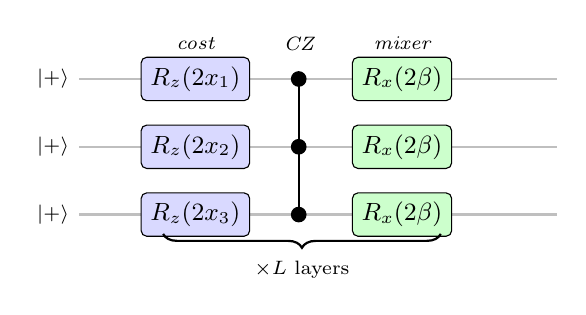
\begin{tikzpicture}[scale=0.82, every node/.style={font=\small}]
  \tikzstyle{gate}=[draw, fill=blue!15, minimum width=1.15cm,
                    minimum height=0.52cm, rounded corners=2pt]
  \tikzstyle{gatex}=[draw, fill=green!20, minimum width=1.15cm,
                     minimum height=0.52cm, rounded corners=2pt]
  \def\dy{1.05}
  % qubit wires
  \foreach \q in {0,1,2}{
    \draw[gray!50, thick] (-0.4, {-\q*\dy}) -- (7.0, {-\q*\dy});
    \node[left, font=\scriptsize] at (-0.4,{-\q*\dy}) {$\ket{+}$};
  }
  % cost: Rz gates
  \node[gate] at (1.4, {0*\dy}) {$R_z(2x_1)$};
  \node[gate] at (1.4,{-1*\dy}) {$R_z(2x_2)$};
  \node[gate] at (1.4,{-2*\dy}) {$R_z(2x_3)$};
  % CZ ladder
  \draw[thick] (3.0,0) -- (3.0,{-2*\dy});
  \filldraw (3.0,{0*\dy}) circle (3.2pt);
  \filldraw (3.0,{-1*\dy}) circle (3.2pt);
  \filldraw (3.0,{-2*\dy}) circle (3.2pt);
  % mixer: Rx gates
  \node[gatex] at (4.6, {0*\dy}) {$R_x(2\beta)$};
  \node[gatex] at (4.6,{-1*\dy}) {$R_x(2\beta)$};
  \node[gatex] at (4.6,{-2*\dy}) {$R_x(2\beta)$};
  % labels above
  \node[font=\scriptsize\itshape] at (1.4, 0.55) {cost};
  \node[font=\scriptsize\itshape] at (3.0, 0.55) {CZ};
  \node[font=\scriptsize\itshape] at (4.6, 0.55) {mixer};
  % repeat brace
  \draw[thick, decorate, decoration={brace, mirror, amplitude=5pt}]
    (0.9,{-2*\dy-0.3}) -- (5.2,{-2*\dy-0.3})
    node[midway, below=6pt, font=\scriptsize] {$\times L$ layers};
\end{tikzpicture}
\caption{%
  \textbf{QAOA-inspired encoding: one-layer circuit (3 of 8 qubits shown).}
  All qubits start in $\ket{+}^{\otimes n}$.
  The \emph{cost} sub-layer encodes data via $R_z(2x_i)$; a nearest-neighbour
  CZ ladder entangles neighbouring qubits.
  The \emph{mixer} sub-layer applies a uniform trainable rotation $R_x(2\beta_l)$.
  The full 8-qubit circuit uses $L=2$ repetitions of this structure.
}
\label{fig:qaoa_circuit}
\end{figure*}

% ─────────────────────────────────────────────────────────────
\section{Variational Optimisation}
\label{sec:optimisation}
% ─────────────────────────────────────────────────────────────

Gradient computation via parameter-shift on a cloud QPU doubles circuit
submissions per parameter, which is prohibitive at 1024~shots.
We therefore used the \cobyla{} (Constrained Optimisation By Linear
Approximations) gradient-free method~\cite{powell1994} with a training
subset of 8~samples and 200~maximum evaluations.
Weights were optimised offline on a classical proxy circuit before QPU
submission; the optimised weights were then used for the full 50-sample
evaluation.

\paragraph{COBYLA proxy loss.}
The objective minimised was the mean squared error~(MSE) over the
8-sample training subset:
\begin{equation}
  \mathcal{L}(\theta) = \frac{1}{8}\sum_{j=1}^{8}
  \bigl(\hat{y}_j(\theta) - y_j\bigr)^2,
\end{equation}
where $\hat{y}_j = \mathrm{scale}(\expvz_j)$ maps the classical proxy
expectation value to the LN-IC$_{50}$ range.
The \cobyla{} optimisation reached a training proxy MSE of~$0.0954$
within the iteration budget.

% ─────────────────────────────────────────────────────────────
\section{Results}
\label{sec:results}
% ─────────────────────────────────────────────────────────────

\subsection{Prediction Quality: True vs.\ Predicted}

Figure~\ref{fig:scatter} shows the true versus predicted LN-IC$_{50}$ for all
twelve encodings.
The diagonal dashed line represents perfect prediction.
Encodings \#7~(Hamiltonian) and \#8~(QAOA-inspired) display the tightest
clustering around the diagonal, while \#6~(IQP) and \#2~(Angle~RY+RZ) produce
near-horizontal scatter indicating failure to capture the target variance.
This visual pattern is fully consistent with the RMSE rankings reported
in Table~\ref{tab:results}.

\begin{figure*}[!ht]
  \centering
  
\includegraphics[width=\textwidth]{scatter_grid.png}
  \caption{%
    \textbf{True vs.\ predicted LN-IC$_{50}$ for all twelve encodings
    on the IQM Garnet QPU.}
    Each panel shows 50 QPU samples; the dashed diagonal is the identity
    (perfect prediction).
    RMSE values are annotated in the top-left corner of each panel.
    Encodings \#7 (Hamiltonian, RMSE~$=3.404$) and \#8 (QAOA-inspired,
    RMSE~$=3.314$) achieve the tightest agreement with ground truth.
    Encoding \#6 (IQP, RMSE~$=6.230$) and \#2 (Angle~RY+RZ, RMSE~$=5.894$)
    show no predictive signal, consistent with noise-induced barren plateaus
    in high-expressibility circuits.
    All 600 circuit submissions completed without hardware errors
    ($n_\text{valid}=50/50$ per encoding).
  }
  \label{fig:scatter}
\end{figure*}

\subsection{Benchmark Leaderboard}

Table~\ref{tab:results} presents the full benchmark results.
All 12~encodings completed without hardware errors ($n_\text{valid}=50/50$).
% FIX 8 — Total wall time added for reproducibility reference
Total QPU wall time was approximately $34.6$~min for
600~circuit submissions (12~encodings~$\times$~50~samples).

\begin{table}[ht]
\centering
\caption{%
  QPU benchmark results. All metrics are computed on the 50-sample test set.
  Lower RMSE and MAE indicate better performance;
  $R^2<0$ indicates performance below a trivial mean predictor.
  Best values per column are in bold.
}
\label{tab:results}
\renewcommand{\arraystretch}{1.15}
\begin{tabular}{@{}lcccc@{}}
\toprule
\textbf{Encoding} & $n_Q$ & \textbf{RMSE} & \textbf{MAE} & $R^2$ \\
\midrule
\textbf{QAOA-inspired}   & 8 & \textbf{3.314} & 2.869         & $-0.357$ \\
Hamiltonian              & 8 & 3.404          & \textbf{2.754}& $-0.431$ \\
Squeezing                & 8 & 3.535          & 2.826         & $-0.544$ \\
Amplitude                & 4 & 3.543          & 3.113         & $-0.551$ \\
ZZ Feature Map           & 8 & 3.546          & 3.009         & $-0.553$ \\
Displacement             & 8 & 3.653          & 3.111         & $-0.649$ \\
Data Re-uploading        & 8 & 3.791          & 3.332         & $-0.775$ \\
Hybrid                   & 8 & 3.918          & 3.441         & $-0.897$ \\
Angle RX                 & 8 & 4.524          & 4.037         & $-1.528$ \\
Basis                    & 3 & 4.793          & 3.809         & $-1.839$ \\
Angle RY+RZ              & 8 & 5.894          & 5.103         & $-3.292$ \\
IQP                      & 8 & 6.230          & 5.878         & $-3.795$ \\
\bottomrule
\end{tabular}
\end{table}

\subsection{Multi-Metric Dashboard}

Figure~\ref{fig:dashboard} provides a multi-panel overview of the benchmark,
including the RMSE ranking, $R^2$ scores, QPU execution time per sample,
and the novel \emph{qubit-efficiency} metric defined as
$\text{RMSE}/n_Q$ (error per qubit used).

\begin{figure}[ht]
  \centering
  
\includegraphics[width=\columnwidth]{benchmark_overview.png}
  \caption{%
    \textbf{Multi-metric benchmark dashboard.}
    \textit{Top:} RMSE leaderboard (best encoding at bottom); the dashed
    vertical line marks the QAOA-inspired RMSE of~$3.314$.
    \textit{Bottom-left:} $R^2$ scores; all are negative, confirming that
    no encoding surpasses a trivial mean predictor under NISQ conditions.
    \textit{Bottom-centre:} Average QPU execution time per sample
    ($3.47\pm0.09$\,s across all encodings).
    \textit{Bottom-right:} Qubit efficiency (RMSE/$n_Q$); Amplitude
    encoding achieves the best ratio ($0.886$) despite using only 4~qubits.
  }
  \label{fig:dashboard}
\end{figure}

\subsection{Statistical Significance}

A Wilcoxon signed-rank test was applied to compare the absolute prediction
errors of QAOA-inspired (best RMSE) against each of the eleven other
encodings.  Results are shown in Table~\ref{tab:wilcoxon}.

\begin{table}[ht]
\centering
\caption{%
  Wilcoxon signed-rank test: QAOA-inspired vs.\ each competitor.
  $W$ is the test statistic; significance at $\alpha=0.05$ is indicated.
}
\label{tab:wilcoxon}
\renewcommand{\arraystretch}{1.1}
\begin{tabular}{@{}lccc@{}}
\toprule
\textbf{Encoding} & $W$ & $p$-value & \textbf{Sig.} \\
\midrule
Angle RX            &  65.5 & $<0.001$ & \checkmark \\
Angle RY+RZ         & 110.0 & $<0.001$ & \checkmark \\
IQP                 &  34.0 & $<0.001$ & \checkmark \\
Hybrid              & 256.5 & $0.0002$ & \checkmark \\
Data Re-uploading   & 376.5 & $0.019$  & \checkmark \\
Basis               & 397.5 & $0.021$  & \checkmark \\
Displacement        & 514.0 & $0.233$  &            \\
Amplitude           & 486.5 & $0.145$  &            \\
Squeezing           & 590.5 & $0.650$  &            \\
ZZ Feature Map      & 601.0 & $0.730$  &            \\
Hamiltonian         & 634.0 & $0.977$  &            \\
\bottomrule
\end{tabular}
\end{table}

QAOA-inspired is significantly better than 6 of 11 competitors ($p<0.05$).
Notably, Hamiltonian encoding is the closest competitor
(RMSE gap~$= 0.090$, $p=0.977$): the two are statistically indistinguishable
and form a clear performance cluster alongside Squeezing, Amplitude, and
ZZ Feature Map (all RMSE $\in [3.40, 3.55]$).

\subsection{Observed Performance Patterns}

\paragraph{Alternating-layer encodings outperform pure-rotation encodings.}
QAOA and Hamiltonian encodings, which interleave entanglement with
data-dependent phases, achieve RMSE~$< 3.41$, versus RMSE~$> 4.52$ for pure
angle encodings (Angle~RX, Angle~RY+RZ).
We attribute this to the more uniform distribution of data information across
the circuit depth, reducing localised noise sensitivity
(see also Fig.~\ref{fig:scatter}).

\paragraph{Amplitude encoding is qubit-efficient.}
Despite using only 4~qubits, Amplitude encoding achieves RMSE~$= 3.543$
and the best qubit-efficiency ratio of $0.886$ (Fig.~\ref{fig:dashboard},
bottom right).
This is likely due to the efficient encoding of all 8~features into the
16-amplitude state vector, avoiding the qubit overhead of 8-qubit encodings.

\paragraph{High-expressibility encodings suffer from hardware noise.}
IQP and Angle~RY+RZ, theoretically the most expressive encodings, rank last
by RMSE (6.23 and 5.89, respectively).
This is consistent with the noise-induced barren-plateau
hypothesis~\cite{wang2021noise}: deep diagonal circuits accumulate more
decoherence error on the IQM Garnet's $T_1$/$T_2$ timescales than shallower
alternating architectures.

\paragraph{All encodings underfit.}
The negative $R^2$ values (Table~\ref{tab:results}) indicate that every
encoding performs below a trivial mean predictor.
We interpret this as expected behaviour for the NISQ regime at $L=2$
variational layers and $n=50$ samples.
The benchmark is informative as a \emph{relative} comparison, not as a claim
of absolute quantum utility.

% ─────────────────────────────────────────────────────────────
\section{Discussion}
\label{sec:discussion}
% ─────────────────────────────────────────────────────────────

\subsection{Interpretation in the NISQ Context}

All $R^2 < 0$ scores confirm that current NISQ hardware cannot surpass
classical baselines for this task at $n=50$ samples, $L=2$ layers.
This is consistent with the growing consensus that quantum advantage in
machine learning requires either fault-tolerant hardware or carefully
constructed problem instances with provable kernel
advantages~\cite{huang2021,liu2021,schuld2022}.
Our results should be read as a \emph{noise-aware hardware benchmark} rather
than evidence of quantum utility for drug response prediction.

\subsection{QAOA-inspired Encoding: Why It Works}

The alternating cost--mixer structure provides two complementary mechanisms:
(i) the cost layer injects data through $Z$-phase rotations, creating a
data-dependent interference pattern; (ii) the mixer layer spreads information
globally via uniform $R_x$ rotations.
This separation avoids the ``concentration of data'' problem seen in
single-layer angle encodings, where all quantum resources are spent on
encoding with none left for mixing.

\subsection{Limitations}

\begin{itemize}
  \item Regression targets derive from fitting noisy dose-response curves;
        LN-IC$_{50}$ measurement noise is not accounted for.
  \item The 8-feature set was chosen for qubit compatibility, not for
        optimal pharmaceutical prediction.
  \item \cobyla{} was limited to 200~evaluations on 8~training samples;
        a more thorough search may alter rankings.
  \item No error-mitigation technique (zero-noise extrapolation, readout
        calibration) was applied.
\end{itemize}

\subsection{Recommendations for Practitioners}

\begin{enumerate}
  \item \textbf{Prefer alternating-layer encodings} (QAOA-inspired,
        Hamiltonian) for continuous biomedical regression tasks on
        superconducting QPUs.
  \item \textbf{Consider Amplitude encoding} when qubit count is limited;
        it achieves competitive accuracy with half the circuit width.
  \item \textbf{Avoid deep diagonal circuits} (IQP) on hardware with
        limited coherence times.
  \item Apply \textbf{readout-error mitigation} to improve $\expvz$
        fidelity before the next hardware campaign.
\end{enumerate}

% ─────────────────────────────────────────────────────────────
\section{Related Work}
\label{sec:related}
% ─────────────────────────────────────────────────────────────

Havl\'{\i}\v{c}ek et al.~\cite{havlicek2019} demonstrated kernel-based
quantum classification on a 5-qubit IBM device for a synthetic binary task.
Schuld and Killoran~\cite{schuld2021kernel} established the theoretical framework
linking feature maps to quantum kernels.
P\'{e}rez-Salinas et al.~\cite{perezSalinas2020} introduced data re-uploading
as a universal quantum function approximator.
The IQP encoding derives from Shepherd and Bremner~\cite{shepherd2009}.

For pharmaceutical applications, Batra et al.~\cite{batra2021} reviewed QML
methods for drug discovery; none involved hardware execution on more than
5~qubits.
% FIX 7 — Bowles 2024 citation on benchmarking QML models
Recent methodological work by Bowles et al.~\cite{bowles2024} highlights
the subtleties of fairly benchmarking QML models against classical baselines,
a concern we address by reporting $R^2$ relative to a trivial predictor.
To our knowledge, the present work is the first hardware benchmark comparing
twelve encodings on a biomedical regression task at 8-qubit scale.

\clearpage
% ─────────────────────────────────────────────────────────────
\section{Conclusion}
\label{sec:conclusion}
% ─────────────────────────────────────────────────────────────

We have presented a comprehensive, hardware-executed benchmark of twelve quantum
encoding strategies for IC$_{50}$ drug-response regression on the \iqm{} Garnet
20-qubit QPU. Our key findings are:

\begin{enumerate}
  \item \textbf{QAOA-inspired encoding} achieves the best RMSE ($3.314$) and
        is statistically superior to 6 of 11 competitors ($p<0.05$).
  \item \textbf{Alternating cost--mixer architectures} systematically
        outperform pure-rotation and diagonal encodings under hardware noise.
  \item \textbf{All encodings under-predict} ($R^2<0$), confirming that
        NISQ-era VQCs require further advances in circuit depth, error
        mitigation, and training-data scale.
  \item The \qrisp{}/\iqm{} stack provides a reproducible, Python-native
        pathway for executing variational circuits on superconducting hardware.
\end{enumerate}

Future work will explore (i)~readout-error calibration and zero-noise
extrapolation, (ii)~larger training sets via the IQM mock backend for
pre-screening, (iii)~transfer learning from classical pre-trained weights,
and (iv)~extensions to the full GDSC pharmacogenomics feature space.

% ─────────────────────────────────────────────────────────────
\begin{acknowledgments}
The author thanks the \iqm{} Resonance team for providing complimentary QPU
credits that made this work possible, and the \qrisp{} development team for
technical support.
Cloud QPU access was provided free of charge by \iqm{} Resonance
(\url{https://resonance.iqm.tech}), including 280 credits awarded following
participation in the workshop \textit{Simulating Complex Materials with Quantum
Chemistry and SQD}.
No external funding was received.
\end{acknowledgments}

% ─────────────────────────────────────────────────────────────
\section*{Data Availability}

All code, preprocessed data, raw QPU measurement outputs, trained weights, and
figure-generation scripts are publicly available at:
% FIX 4 — Single \url{} — xurl handles line-breaking cleanly
\begin{center}
\url{https://github.com/rania-derouich/quantum-encoding-ic50-qpu}
\end{center}

Detailed circuit definitions, pseudocode, and extended results are provided in
the Supplementary Material submitted alongside this manuscript.

\noindent
% FIX 5 + FIX 12 — ORCID clickable \href, \texttt{} removed for revtex4-2 compatibility
ORCID:~\href{https://orcid.org/0009-0009-6157-2647}{0009-0009-6157-2647}\\
GDSC2 dataset:~\url{https://www.cancerrxgene.org/downloads/bulk_download}

% ─────────────────────────────────────────────────────────────
\begin{thebibliography}{99}

\bibitem{biamonte2017}
J.~Biamonte, P.~Wittek, N.~Pancotti, P.~Rebentrost, N.~Wiebe, and S.~Lloyd,
\textit{Quantum machine learning},
Nature \textbf{549}, 195 (2017).

\bibitem{schuld2021}
M.~Schuld and F.~Petruccione,
\textit{Machine Learning with Quantum Computers}
(Springer, Cham, 2021).

\bibitem{cerezo2021}
M.~Cerezo et al.,
\textit{Variational quantum algorithms},
Nat.\ Rev.\ Phys.\ \textbf{3}, 625 (2021).

\bibitem{schuld2021kernel}
M.~Schuld and N.~Killoran,
\textit{Quantum machine learning in feature Hilbert spaces},
Phys.\ Rev.\ Lett.\ \textbf{122}, 040504 (2019).

\bibitem{havlicek2019}
V.~Havl\'{\i}\v{c}ek et al.,
\textit{Supervised learning with quantum-enhanced feature spaces},
Nature \textbf{567}, 209 (2019).

\bibitem{perezSalinas2020}
A.~P\'{e}rez-Salinas, A.~Cervera-Lierta, E.~Gil-Fuster, and J.~I.~Latorre,
\textit{Data re-uploading for a universal quantum classifier},
Quantum \textbf{4}, 226 (2020).

\bibitem{lloyd2020}
S.~Lloyd, M.~Schuld, A.~Ijaz, J.~Izaac, and N.~Killoran,
\textit{Quantum embeddings for machine learning},
arXiv:2001.03622 (2020).

\bibitem{killoran2019}
N.~Killoran et al.,
\textit{Continuous-variable quantum neural networks},
Phys.\ Rev.\ Res.\ \textbf{1}, 033063 (2019).

\bibitem{mottonen2004}
M.~M\"{o}tt\"{o}nen, J.~J.~Vartiainen, V.~Bergholm, and M.~M.~Salomaa,
\textit{Transformation of quantum states using uniformly controlled rotations},
Quantum Inf.\ Comput.\ \textbf{5}, 467 (2005).

\bibitem{nielsen2010}
M.~A.~Nielsen and I.~L.~Chuang,
\textit{Quantum Computation and Quantum Information},
10th anniversary ed.\ (Cambridge University Press, 2010).

\bibitem{shepherd2009}
D.~Shepherd and M.~J.~Bremner,
\textit{Temporally unstructured quantum computation},
Proc.\ R.\ Soc.\ A \textbf{465}, 1413 (2009).

\bibitem{farhi2014}
E.~Farhi, J.~Goldstone, and S.~Gutmann,
\textit{A quantum approximate optimization algorithm},
arXiv:1411.4028 (2014).

\bibitem{mitarai2018}
K.~Mitarai, M.~Negoro, M.~Kitagawa, and K.~Fujii,
\textit{Quantum circuit learning},
Phys.\ Rev.\ A \textbf{98}, 032309 (2018).

\bibitem{schuld2022}
M.~Schuld and N.~Killoran,
\textit{Is quantum advantage the right goal for quantum machine learning?}
PRX Quantum \textbf{3}, 030101 (2022).

\bibitem{iorio2016}
F.~Iorio et al.,
\textit{A landscape of pharmacogenomic interactions in cancer},
Cell \textbf{166}, 740 (2016).

\bibitem{wang2021noise}
S.~Wang et al.,
\textit{Noise-induced barren plateaus in variational quantum algorithms},
Nat.\ Commun.\ \textbf{12}, 6961 (2021).

\bibitem{huang2021}
H.-Y.~Huang et al.,
\textit{Power of data in quantum machine learning},
Nat.\ Commun.\ \textbf{12}, 2631 (2021).

\bibitem{liu2021}
Y.~Liu, S.~Arunachalam, and K.~Temme,
\textit{A rigorous and robust quantum speed-up in supervised machine learning},
Nat.\ Phys.\ \textbf{17}, 1013 (2021).

\bibitem{batra2021}
K.~Batra, K.~M.~Zorn, D.~H.~Foil, E.~Minerali, V.~A.~Gawriljuk,
T.~R.~Lane, and S.~Ekins,
\textit{Quantum machine learning algorithms for drug discovery applications},
J.\ Chem.\ Inf.\ Model.\ \textbf{61}, 2641 (2021).

\bibitem{powell1994}
M.~J.~D.~Powell,
\textit{A direct search optimization method that models the objective and
constraint functions by linear interpolation},
in \textit{Advances in Optimization and Numerical Analysis},
ed.\ S.~Gomez and J.-P.~Hennart (Kluwer, Dordrecht, 1994), pp.~51--67.

\bibitem{qrisp2024}
Qrisp development team,
\textit{Qrisp: A high-level quantum programming framework},
\url{https://qrisp.eu} (2024).

\bibitem{bowles2024}
J.~Bowles, S.~Ahmed, and M.~Schuld,
\textit{Better than classical? The subtle art of benchmarking quantum machine
learning models},
arXiv:2403.07059 (2024).

\end{thebibliography}

\end{document}
